\documentclass{beamer}

%%%%%%%%%%%%%%%%%%%%%%%%%%%%%%%%%%%%%%%%%%%%%%%%%%%%%%%%%%%%%%%%
%%%                  Themes and such                         %%%
%%%%%%%%%%%%%%%%%%%%%%%%%%%%%%%%%%%%%%%%%%%%%%%%%%%%%%%%%%%%%%%%
\mode<presentation>
{
  %\usetheme{Copenhagen}  
  %\usetheme{Warsaw}  
  \usetheme{Malmoe}  
%    \setbeamertemplate{headline}{}
  %make my huge toc fit on one slide (and not look horrible)
  %\setbeamerfont{subsection in toc}{series=\bfseries}
  %\setbeamerfont{subsection in toc}{size=\tiny,series=\bfseries}
}

%%%%%%%%%%%%%%%%%%%%%%%%%%%%%%%%%%%%%%%%%%%%%%%%%%%%%%%%%%%%%%%%
%%%                       Packages                           %%%
%%%%%%%%%%%%%%%%%%%%%%%%%%%%%%%%%%%%%%%%%%%%%%%%%%%%%%%%%%%%%%%%
\usepackage{multimedia}
\usepackage{multirow}
\usepackage{subfigure}
\usepackage{amsmath}

% Define commands
 \newcommand{\half}{\ensuremath{\frac{1}{2}}}

 \newcommand{\bea}{\begin{eqnarray}}
 \newcommand{\eea}{\end{eqnarray}}
 \newcommand{\beq}{\begin{equation}}
 \newcommand{\eeq}{\end{equation}}
 \newcommand{\bed}{\begin{displaymath}}
 \newcommand{\eed}{\end{displaymath}}

 \newcommand{\pd}[2]{\frac{\partial #1}{\partial #2}}
 \newcommand{\pf}[2]{\frac{d #1}{d #2}}
 \newcommand{\pdt}[2]{\frac{\partial^2 #1}{\partial #2^2}}
 \newcommand{\pft}[2]{\frac{d^2 #1}{d #2^2}}
 \newcommand{\pdtno}[2]{\frac{\partial^2 #1}{\partial #2}}
 \newcommand{\pdd}[3]{\frac{\partial^2 #1}{\partial #2 \partial #3}}
 \newcommand{\pff}[3]{\frac{d^2 #1}{d #2 d #3}}

 \graphicspath{{../figures/}}


%%%%%%%%%%%%%%%%%%%%%%%%%%%%%%%%%%%%%%%%%%%%%%%%%%%%%%%%%%%%%%%%
%%%                     Title Info                           %%%
%%%%%%%%%%%%%%%%%%%%%%%%%%%%%%%%%%%%%%%%%%%%%%%%%%%%%%%%%%%%%%%%

\title[\hspace{-0.2cm} Time Dependent Discrete Adjoint]
{
Time Dependent Discrete Adjoint Formulations for Structural Dynamics
}

\author[Komahan Boopathy]
{
  \Large {Komahan Boopathy}\\
}

\institute
{
  \large Georgia Institute of Technology\\
 School of Aerospace Engineering\\
 Atlanta, GA
}

\date
{
\small \today
}

\begin{document}

\begin{frame}
  \titlepage
\end{frame}

%\begin{frame}
%  \frametitle{Outline}
%  \tableofcontents
%\end{frame}

\begin{frame}[allowframebreaks] \frametitle{Newmark--Beta--Gamma Method Adjoint}

  \tiny{We are interested in finding the derivative of time-averaged
    function 
    \begin{equation}\label{eqn:time-averaged-function}
      F = \frac{1}{T}\int_{0}^T f_k(\ddot{q}_k, \dot{q}_k,
      q_k, t_k , x)~dt=\sum_{k=0}^N h f_k,
    \end{equation} 
with respect to the design variables $x$, such that the governing
equations are satisfied at all time steps, i.e., their corresponding
residuals must be zero:
\begin{equation}\label{eqn:nbg-residual}
  R_k=R_k(\ddot{q}_k, \dot{q}_k, q_k, t_k , x) = 0.
\end{equation}
 We use Newmark--Beta--Gamma (NBG) time-marching method to integrate
 and solve for the states over time. The states are approximated as
 follows:
\begin{equation}\label{eqn:nbg-approx-qdot}
     S_k = S_k(\ddot{q}_{k}, \ddot{q}_{k-1}, \underline{\dot{q}_k}, \dot{q}_{k-1}) =  \dot{q}_{k-1}  + (1-\gamma) h \ddot{q}_{k-1} +  \gamma h \ddot{q}_{k}- \dot{q}_k=0, 
\end{equation}
\begin{equation}\label{eqn:nbg-approx-q}
     T_k = T_k(\ddot{q}_{k}, \ddot{q}_{k-1}, \underline{{q}_k}, {q}_{k-1}) = {q}_{k-1} + h \dot{q}_{k-1} +\frac{1-2\beta}{2}
    h^2\ddot{q}_{k-1} + \beta h^2 \ddot{q}_k-{q}_k=0, 
\end{equation}
where $\beta$ and $\gamma$ are the coefficients from NBG method. The
acceleration states $\ddot{q}_k$ are the primary unknown at each time
step from which the velocity and position states are estimated.

    \framebreak

    We introduce $\rho_k$, $\sigma_k$ and $\tau_k$ as the adjoint
    variables associated with each of these ``constraint'' equations
    and the Lagrangian function is written as:
    \begin{equation}\label{eqn:nbg-lagrangian}
      {\cal{L}} = \sum_{k=0}^N h f_k+ \sum_{k=0}^N h \rho_k^T R_k + \sum_{k=0}^N \sigma_k^T S_k + \sum_{k=0}^N \tau_k^T T_k.
    \end{equation} 
    The auxiliary equations $S_k$ and $T_k$ are independent of the
    design variables $x$, therefore, the total derivative can be
    written as a linear combination of contributions from the function
    of interest and the constraint:
    \begin{equation}\label{eqn:nbg-total-derivative}
      \pd{\cal{L}}{x} = \pd{F}{x} = \sum_{k=0}^N h \pd{f_k}{x}^T + \sum_{k=0}^N h
    \pd{R_k}{x}^T \lambda_k.
    \end{equation}

    The conditions $$\pd{\cal{L}}{{q}_k}, \pd{\cal{L}}{\dot{q}_k},
    \pd{\cal{L}}{\ddot{q}_k} = 0$$ can be used to generate a coupled
    system of equations to solve \underline{simultaneously} for the
    adjoint variables at each time step. Since the equations $S_k$ and
    $T_k$ are explicit, it becomes possible to solve
    \underline{sequentially} for the adjoint variables at each step. This property
    is beneficial in terms of reducing the size of the linear system.
    The steps involved are detailed as follows.
         Setting $\pd{\cal{L}}{{q}_k} = 0$ yields:
         \begin{equation}
           \begin{split}
             \tau_k = \tau_{k+1} + \left\{h \pd{f_{k+1}}{{q}_{k+1}} \right\}^T + \left[ h \pd{R_{k+1}}{{q}_{k+1}} \right]^T \rho_{k+1}  
           \end{split}
         \end{equation}

    Setting $\pd{\cal{L}}{\dot{q}_k} = 0$ yields:
         \begin{equation}
           \begin{split}
             \sigma_k = \sigma_{k+1} + h \tau_{k+1}  + \left\{ h \pd{f_{k+1}}{\dot{q}_{k+1}} +  h^2 \pd{f_{k+1}}{{q}_{k+1}} \right\}^T + \left[ h \pd{R_{k+1}}{\dot{q}_{k+1}} +  h^2 \pd{R_{k+1}}{{q}_{k+1}} \right]^T \rho_{k+1} 
           \end{split}
         \end{equation}
         
    Figure~\ref{fig:nbg-illustration} shows the flow of information across
    states.
    \begin{figure}
      \centering
      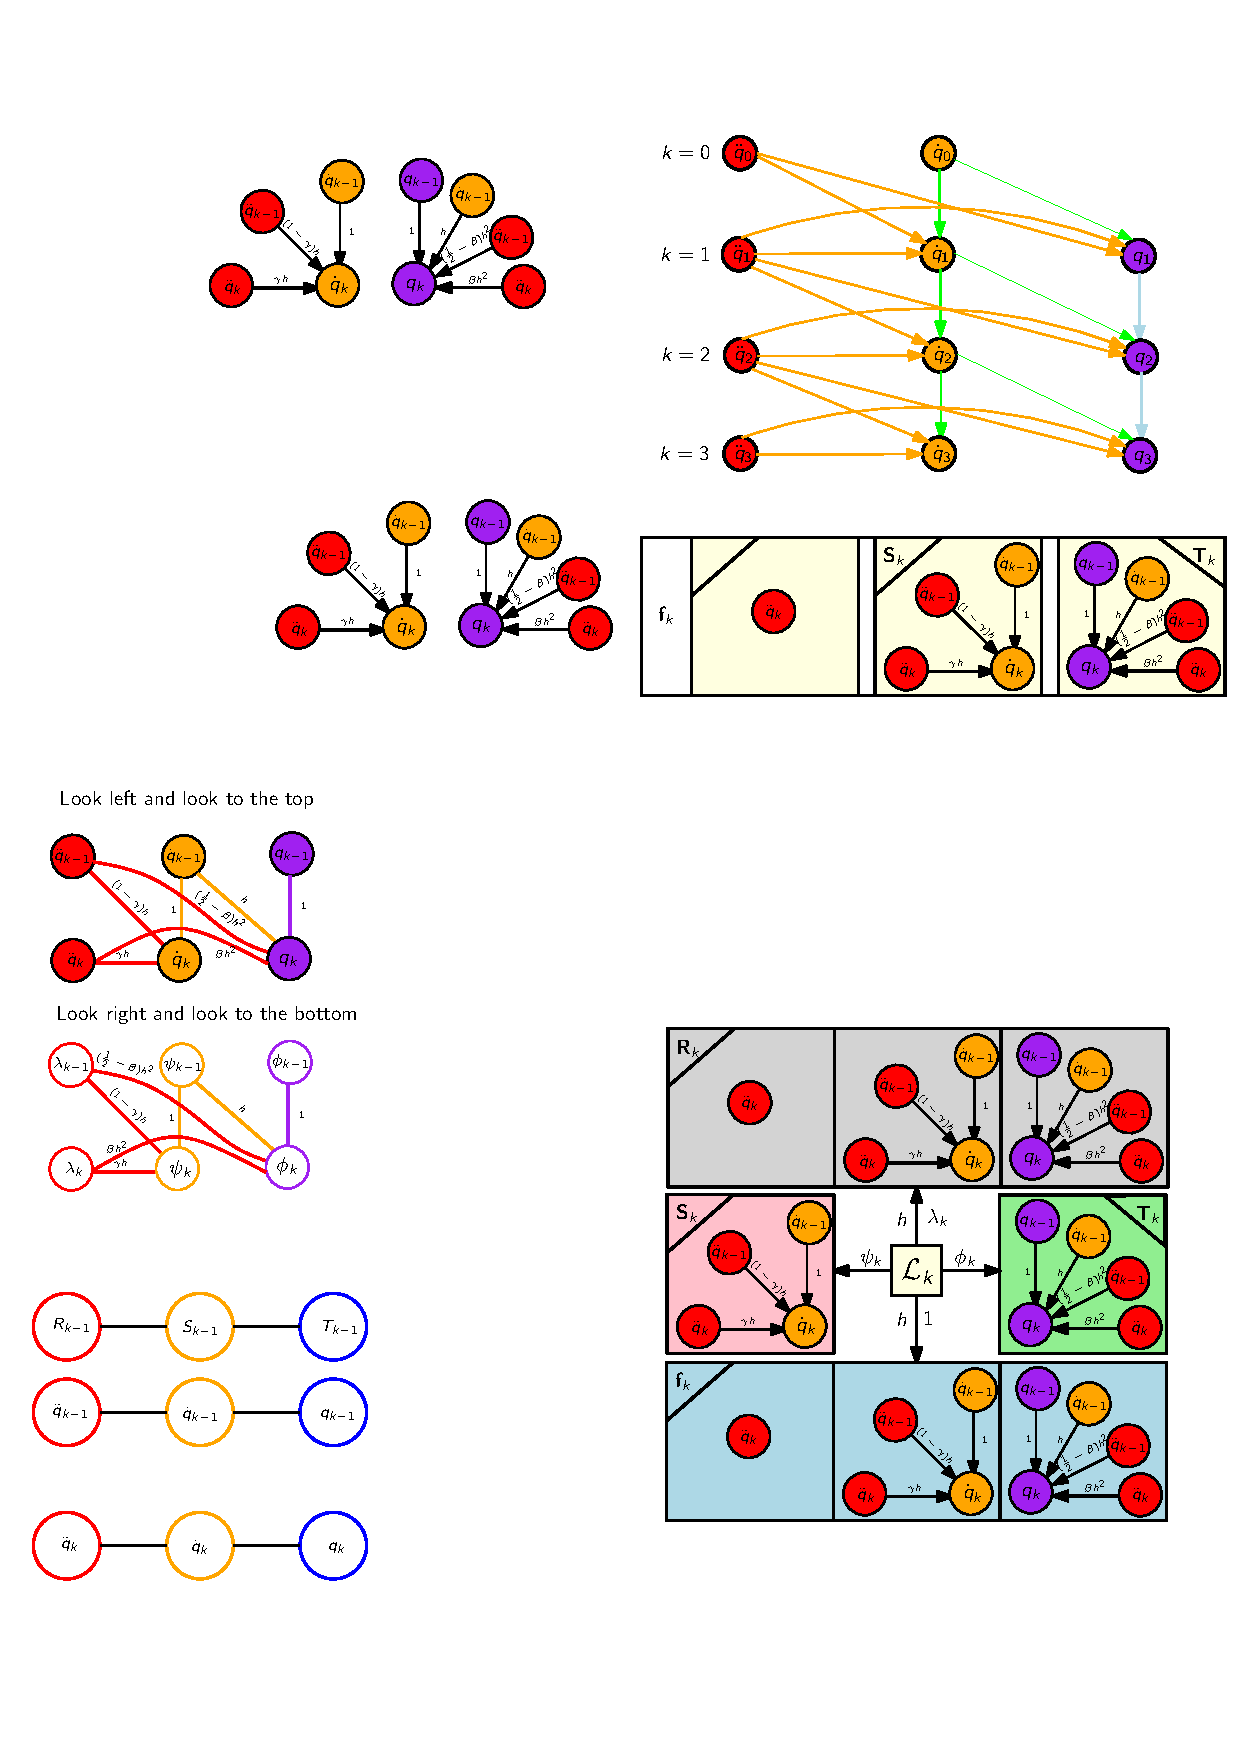
\includegraphics[width=\textwidth]{nbg-chart.pdf}
      %\caption{Illustrations showing the working of NBG method.}
      \label{fig:nbg-illustration}
    \end{figure}

         Setting $\pd{\cal{L}}{\ddot{q}_k} = 0$ yields:
         \begin{equation}
           \begin{split}
             \left[ \pd{R_k}{\ddot{q}_k} + \gamma h \pd{R_k}{\dot{q}_k} + \beta h^2 \pd{R_k}{{q}_k} \right]^T \rho_k = &- \left\{ \pd{f_k}{\ddot{q}_k} + \gamma h \pd{f_k}{\dot{q}_k} + \beta h^2 \pd{f_k}{{q}_k} \right\}^T \\
             & -  \frac{1}{h}\left\{  \gamma h  \sigma_k + \beta h^2   \tau_k \right\}^T\\
             & -  \left\{ (1-\gamma) h \pd{f_{k+1}}{\dot{q}_{k+1}} + \frac{1-2\beta}{2} h^2 \pd{f_{k+1}}{{q}_{k+1}} \right\}^T \\
                          & -  \left[ (1-\gamma) h \pd{R_{k+1}}{\dot{q}_{k+1}} + \frac{1-2\beta}{2} h^2 \pd{R_{k+1}}{{q}_{k+1}} \right]^T\rho_{k+1} \\
             & -  \frac{1}{h} \left\{ (1-\gamma) h \sigma_{k+1} + \frac{1-2\beta}{2} h^2 \tau_{k+1} \right\}^T\\
           \end{split}
         \end{equation}

}
\end{frame}

\end{document}

%         We explore further simplifications by substituting equations.
%
%         \begin{equation}
%           \begin{split}
%             \left[ \frac{1}{h^2} \pd{R_k}{\ddot{q}_k} + \gamma \frac{1}{h} \pd{R_k}{\dot{q}_k} + \beta \pd{R_k}{{q}_k} \right]^T \rho_k = &- \left\{ \frac{1}{h^2}  \pd{f_k}{\ddot{q}_k} + \gamma \frac{1}{h} \pd{f_k}{\dot{q}_k} + \beta \pd{f_k}{{q}_k} \right\}^T \\
%             & -  \frac{1}{h}\left\{  \gamma \frac{1}{h}  \left( \sigma_{k+1} + h \tau_{k+1}  + \left\{ h \pd{f_{k+1}}{\dot{q}_{k+1}} +  h^2 \pd{f_{k+1}}{{q}_{k+1}} \right\}^T + \left[ h \pd{R_{k+1}}{\dot{q}_{k+1}} +  h^2 \pd{R_{k+1}}{{q}_{k+1}} \right]^T \rho_{k+1}  \right) \right\}^T \\
%             & -  \frac{1}{h}\left\{  \beta  \left( \tau_{k+1} + \left\{h \pd{f_{k+1}}{{q}_{k+1}} \right\}^T + \left[ h \pd{R_{k+1}}{{q}_{k+1}} \right]^T \rho_{k+1}  \right) \right\}^T\\
%             & -  \left\{ (1-\gamma) \frac{1}{h} \pd{f_{k+1}}{\dot{q}_{k+1}} + \frac{1-2\beta}{2} \pd{f_{k+1}}{{q}_{k+1}} \right\}^T \\
%             & -  \left[ (1-\gamma) \frac{1}{h} \pd{R_{k+1}}{\dot{q}_{k+1}} + \frac{1-2\beta}{2} \pd{R_{k+1}}{{q}_{k+1}} \right]^T\rho_{k+1} \\
%             & -  \frac{1}{h} \left\{ (1-\gamma) \frac{1}{h} \sigma_{k+1} + \frac{1-2\beta}{2} \tau_{k+1} \right\}^T\\
%           \end{split}
%         \end{equation}
%
%         \framebreak


         \framebreak
        
         Grouping the terms together we get:

         \begin{equation}
           \begin{split}
             \left[ \frac{1}{h^2} \pd{R_k}{\ddot{q}_k} + \gamma \frac{1}{h} \pd{R_k}{\dot{q}_k} + \beta \pd{R_k}{{q}_k} \right]^T \rho_k = &- \left\{ \frac{1}{h^2}  \pd{f_k}{\ddot{q}_k} + \gamma \frac{1}{h} \pd{f_k}{\dot{q}_k} + \beta \pd{f_k}{{q}_k} \right\}^T \\
             & -  \left\{  \gamma \frac{1}{h}  \pd{f_{k+1}}{\dot{q}_{k+1}} +  \gamma \pd{f_{k+1}}{{q}_{k+1}} \right\}^T \\ 
             & -  \left[  \gamma \frac{1}{h}  \pd{R_{k+1}}{\dot{q}_{k+1}} + \gamma \pd{R_{k+1}}{{q}_{k+1}} \right]^T \rho_{k+1}  \\
             & -  \left\{ \beta \pd{f_{k+1}}{{q}_{k+1}} \right\}^T \\ 
             & - \left[  \beta\pd{R_{k+1}}{{q}_{k+1}} \right]^T \rho_{k+1}  \\
             & -  \left\{ (1-\gamma) \frac{1}{h} \pd{f_{k+1}}{\dot{q}_{k+1}} + (\frac{1}{2}-\beta) \pd{f_{k+1}}{{q}_{k+1}} \right\}^T \\
             & -  \left[ (1-\gamma) \frac{1}{h} \pd{R_{k+1}}{\dot{q}_{k+1}} + (\frac{1}{2}-\beta) \pd{R_{k+1}}{{q}_{k+1}} \right]^T\rho_{k+1} \\
             & -  \frac{1}{h} \left\{ \frac{1}{h} \sigma_{k+1} + (\frac{1}{2} +\gamma) \tau_{k+1} \right\}^T\\
           \end{split}
         \end{equation}
        
         \begin{equation}
           \begin{split}
             \left[ \frac{1}{h^2} \pd{R_k}{\ddot{q}_k} + \gamma \frac{1}{h} \pd{R_k}{\dot{q}_k} + \beta \pd{R_k}{{q}_k} \right]^T \rho_k = &- \left\{ \frac{1}{h^2}  \pd{f_k}{\ddot{q}_k} + \gamma \frac{1}{h} \pd{f_k}{\dot{q}_k} + \beta \pd{f_k}{{q}_k} \right\}^T \\
             & -  \left\{  \frac{1}{h} \pd{f_{k+1}}{\dot{q}_{k+1}} +  (\frac{1}{2} +\gamma) \pd{f_{k+1}}{{q}_{k+1}} \right\}^T \\
             & -  \left[  \frac{1}{h} \pd{R_{k+1}}{\dot{q}_{k+1}} +  (\frac{1}{2} +\gamma)  \pd{R_{k+1}}{{q}_{k+1}} \right]^T\rho_{k+1} \\
             & -  \frac{1}{h} \left\{ \frac{1}{h} \sigma_{k+1} + (\frac{1}{2} +\gamma) \tau_{k+1} \right\}^T\\
           \end{split}
         \end{equation}

         Once the primary adjoint variables $\rho_k$ have been
         determined, the total derivative is readily obtained using
         Eq.\eqref{eqn:nbg-total-derivative}:
         $$\pd{\cal{L}}{x} = \pd{F}{x} = \sum_{k=0}^N h \pd{f_k}{x}^T
         + \sum_{k=0}^N h \pd{R_k}{x}^T \rho_k.$$ Notice that
         $\pd{S_k}{x} = \pd{T_k}{x} = 0$.  
  


         We can equivalently scale the equation with $1/h^2$ and represent as follows:
         
         \begin{equation}
           \begin{split}
             \left[ \frac{1}{h^2} \pd{R_k}{\ddot{q}_k} + \gamma \frac{1}{h} \pd{R_k}{\dot{q}_k} + \beta \pd{R_k}{{q}_k} \right]^T \rho_k = &- \left\{ \frac{1}{h^2}  \pd{f_k}{\ddot{q}_k} + \gamma \frac{1}{h} \pd{f_k}{\dot{q}_k} + \beta \pd{f_k}{{q}_k} \right\}^T \\
             & -  \frac{1}{h}\left\{  \gamma \frac{1}{h}  \sigma_k + \beta   \tau_k \right\}^T\\
             & -  \left\{ (1-\gamma) \frac{1}{h} \pd{f_{k+1}}{\dot{q}_{k+1}} + \frac{1-2\beta}{2} \pd{f_{k+1}}{{q}_{k+1}} \right\}^T \\
                          & -  \left[ (1-\gamma) \frac{1}{h} \pd{R_{k+1}}{\dot{q}_{k+1}} + \frac{1-2\beta}{2} \pd{R_{k+1}}{{q}_{k+1}} \right]^T\rho_{k+1} \\
             & -  \frac{1}{h} \left\{ (1-\gamma) \frac{1}{h} \sigma_{k+1} + \frac{1-2\beta}{2} \tau_{k+1} \right\}^T\\
           \end{split}
         \end{equation}
